\section{Description and Methodology}

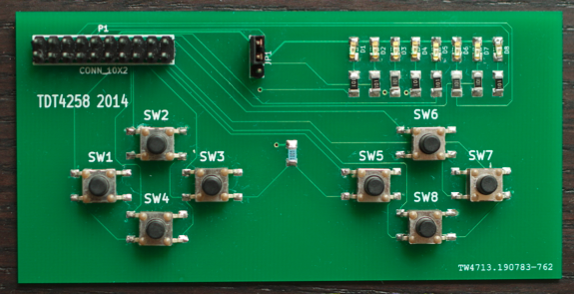
\includegraphics{figures/gamepad.png}



\subsection{Further improvements}
The program described in this report sleeps when it is idle, just waiting for an interrupt.
This is done in the interest of power efficiency.
As described elsewhere, the program sleeps in what is called EM3, where some of the functions are running.
However, a fourth energy mode is available in the microcontroller, and even more power could be saved.

The fourth stage, EM4, is a deep sleep mode where only a few services use power.
After going to EM4, it would take 160 $\mu$s to go back to EM0.
This would be satisfactory for the intended behaviour of the program, and not present much perceived lag when pressing a button.
Unfortunately, to wake up the unit again is limited.
Either the microcontroller needs to be reset, or GPIO interrupt wake must be enabled.
The interrupts for waking up the unit needs to be sent to one of a list of GPIO ports.\cite{referencemanual}

With these limitations, it is clear that the deep sleep mode will not be usuable within the requirements and with the provided hardware.
A small change to the hardware would let the program work as intended, and sleep deeper.
With a multiplexer of all the signals from the buttons, and output to one of the supported GPIO ports, it would be easy to support EM4.
